\documentclass[11pt,aspectratio=169]{beamer}

% Theme
\usetheme{Madrid}
\usecolortheme{default}

% Packages
\usepackage{graphicx}
\usepackage{booktabs}
\usepackage{hyperref}
\usepackage{tikz}
\usepackage{twemojis}
\usetikzlibrary{shapes,arrows,positioning,shadows}

% Title information
\title{Git, GitHub, and VS Code}
\subtitle{Agentic AI for Project Management and Research Productivity}
\author{Tomas Larroucau }
\institute{Arizona State University}
\date{\today}

% Remove navigation symbols
\setbeamertemplate{navigation symbols}{}

% Footer
\setbeamertemplate{footline}[frame number]

\begin{document}

% Title slide
\begin{frame}
\titlepage
\end{frame}

% Table of contents
\begin{frame}{Workshop Overview}
\tableofcontents
\end{frame}

% ============================================================
% SECTION 1: INTRODUCTION
% ============================================================
\section{Introduction}

\begin{frame}{Why This Workshop?}
\begin{columns}[t]
\begin{column}{0.48\textwidth}
\textbf{The Problem:}
\begin{itemize}
    \item Research projects grow messy fast
    % \item ``It worked on my machine'' syndrome
    \item Co-authoring via email and Dropbox can be chaotic
    \item AI tools exist but live \textit{outside} the workflow
\end{itemize}
\end{column}

\begin{column}{0.48\textwidth}
\textbf{What If We Could:}
\begin{itemize}
    \item Work in one environment: code, writing, collaboration
    \item Track every change and undo any mistake
    \item Let AI operate \textit{inside} the project with guardrails
    % \item Automate the boring parts of research
\end{itemize}
\end{column}
\end{columns}

\vfill

\centering
\textbf{Goal:} Set up the infrastructure for truly integrated, AI-assisted research.

\vspace{0.5cm}

\textit{\textbf{``We'll let the AI roam free... but set up proper guardrails.''}}

\vfill
\end{frame}



\begin{frame}{The ``Jur-AI-ssic Park" Approach to Research}
    \centering
    \vspace{0.2cm}
    
    \begin{columns}[t]
        \begin{column}{0.33\textwidth}
            \centering
            \onslide<1->{
                \textbf{\large The Park}\\
                \vspace{0.1cm}
                \textit{(VS Code)}\\
                \vspace{0.3cm}
                % TODO: Replace with AI image: A lush digital jungle island
                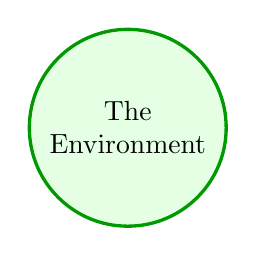
\begin{tikzpicture}
                    \node[circle, draw=green!60!black, fill=green!10, very thick, minimum size=2.5cm, align=center] {The\\Environment};
                \end{tikzpicture}\\
                \vspace{0.3cm}
                \small{The island where everything lives}
            }
        \end{column}
        
        \begin{column}{0.33\textwidth}
            \centering
            \onslide<2->{
                \textbf{\large The Dinosaurs}\\
                \vspace{0.1cm}
                \textit{(AI Agents)}\\
                \vspace{0.3cm}
                % TODO: Replace with AI image: A T-Rex writing code or robot dinosaur
                
\begin{tikzpicture}
                    \node[star, star points=5, draw=red!60!black, fill=red!10, very thick, minimum size=2.5cm, align=center] {Raw\\Power};
                \end{tikzpicture}\\
                \vspace{0.3cm}
                \small{Powerful, fast, but chaotic}
            }
        \end{column}
        
        \begin{column}{0.33\textwidth}
            \centering
            \onslide<3->{
                \textbf{\large The Guardrails}\\
                \vspace{0.1cm}
                \textit{(Git \& GitHub)}\\
                \vspace{0.3cm}
                % TODO: Replace with AI image: High-voltage electric fences
                
\begin{tikzpicture}
                    \node[rectangle, draw=blue!60!black, fill=blue!10, very thick, minimum size=2.5cm, minimum width=2.5cm, align=center] {Safety\\System};
                \end{tikzpicture}\\
                \vspace{0.3cm}
                \small{Keeps the chaos contained}
            }
        \end{column}
    \end{columns}
    
    \vspace{0.8cm}
    \centering
    \onslide<4->{
        \begin{quote}
        \textit{``Your scientists were so preoccupied with whether or not they could, they didn't stop to think if they should... \textbf{Git lets you undo if they shouldn't.}"}
        \end{quote}
    }
\end{frame}

\begin{frame}{The Symbiosis: Agents as Builders}
    \centering
    \begin{columns}[c]
        \begin{column}{0.4\textwidth}
            \centering
            % "The Picture" - Dinosaur building the fence
            \includegraphics[width=\columnwidth]{figures/Symbiosis.png}
        \end{column}
        
        \begin{column}{0.6\textwidth}
            \textbf{From Safety to Superpowers:}
            
            \vspace{0.3cm}
            
            \begin{itemize}
                \itemsep1em
                \item \textbf{VS Code $\rightarrow$ Capability} \\
                \small Agents gain \textit{hands}. They can execute tests, debug, and browse the web.
                
                \item \textbf{Git/GitHub $\rightarrow$ Memory} \\
                \small Issues \& PRs provide persistent context ("Pseudo-Memory") and documentation.
                
                \item \textbf{Agents $\rightarrow$ Mastery} \\
                \small They lower the cost of learning the tools. \\
                \textit{"How do I cherry-pick this commit?"}
            \end{itemize}
        \end{column}
    \end{columns}
\end{frame}

\begin{frame}{What You'll Learn}
    \vspace{0.3cm}
    \begin{itemize}
        \setlength{\itemsep}{0.4cm}
        \item \textbf{VS Code} as integrated development environment
        \item \textbf{Git fundamentals}: commits, branches, merges
        \item \textbf{GitHub workflows}: issues, pull requests, project boards
        \item \textbf{VS Code Chat}: Ask, Edit, and Agent modes
        \item \textbf{GitHub Copilot}: local and cloud workflows
        \item \textbf{AI-assisted} code review and refactoring
        \item \textbf{Complementary tools}: Refine, NotebookLM, Notion
    \end{itemize}
\end{frame}

\begin{frame}{Workshop Materials}
    \vspace{0.3cm}
    \begin{itemize}
        \setlength{\itemsep}{0.4cm}
        \item \textbf{Template Repository}: Complete research project structure
        \item \textbf{Sample Data}: CSV files for demonstration
        \item \textbf{Python Scripts}: Analysis, plotting, table generation
        \item \textbf{LaTeX Templates}: Paper and slides
        \item \textbf{Makefile}: Automated workflow
        \item \textbf{Documentation}: README, agent instructions
    \end{itemize}

\vspace{0.3cm}
Repository available at: \url{https://github.com/tlarroucau/AI_workshop}
\end{frame}

\subsection{Project Structure}

\begin{frame}{Reproducible Research Template}
\hypertarget{main-project-structure}{}
\textbf{Repository Structure:}
\begin{itemize}
    \item \texttt{data/}: Usually only processed data
    \item \texttt{scripts/}: Analysis code
    \item \texttt{output/}: Generated figures and tables
    \item \texttt{tex/}: LaTeX documents (paper, slides)
    \item \texttt{Makefile}: Automation workflow
    \item \texttt{README.md}: Project documentation
    \item \texttt{.gitignore}: Excluded files
\end{itemize}

\vspace{0.3cm}

\textbf{Key Principle:} Everything generated from scripts, nothing manual!

\vspace{0.3cm}
\hyperlink{appendix-makefile}{\beamerbutton{See Makefile slide (Appendix)}}
\end{frame}

\begin{frame}{Workshop Prerequisites}
\begin{columns}[t]
    \begin{column}{0.48\textwidth}
        \textbf{1. Accounts}
        \begin{itemize}
            \item \textbf{GitHub Account}: Create at \url{github.com}
            \item \textbf{Education Benefits}: Apply for student/educator pack at \url{education.github.com} (Upgrade to Pro!)
        \end{itemize}
        
        \vspace{0.2cm}
        
        \textbf{2. Software}
        \begin{itemize}
            \item \textbf{VS Code}: Download from \url{code.visualstudio.com}
            \item \textbf{Git}: Install from \url{git-scm.com}
            \item \textit{Optional}: Python \& LaTeX distribution
        \end{itemize}
    \end{column}

    \begin{column}{0.48\textwidth}
        \textbf{3. Extensions \& Setup}
        \begin{itemize}
            \item \textbf{Link GitHub}: Sign in to GitHub within VS Code (Accounts menu)
            \item \textbf{Copilot}: Install ``GitHub Copilot" extension 
            \item \textbf{MCP Servers}: We will use Github MCP server for integration (I will show how)
        \end{itemize}
        
        \vspace{0.2cm}
        
        \begin{block}{Note on Access}
        GitHub Copilot is now free! However, upgrading to Copilot Pro (via Education pack) offers better models and limits. Verification can take a few days.
        \end{block}
    \end{column}
\end{columns}
\end{frame}



% ============================================================
% SECTION 2: VS CODE
% ============================================================
\begin{frame}[plain]
    \centering
    \vspace{1cm}
    \textbf{\Huge The Environment}
    
    \vspace{0.5cm}
    {\Large Visual Studio Code}
    
    \vspace{1.5cm}
    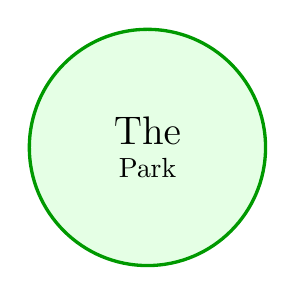
\begin{tikzpicture}
        \node[circle, draw=green!60!black, fill=green!10, very thick, minimum size=3cm, align=center] {\Large The\\Park};
    \end{tikzpicture}
\end{frame}

\section{VS Code: Your Research Environment}

\begin{frame}{What is VS Code?}
\begin{columns}[t]
\begin{column}[t]{0.5\textwidth}
\textbf{Visual Studio Code}
\vspace{0.2cm}
\begin{itemize}
    \setlength{\itemsep}{0.3cm}
    \item Free, open-source editor by Microsoft
    \item Cross-platform (Windows, Mac, Linux)
    \item Extensible via marketplace
    \item Integrated terminal
    \item Built-in Git support
    \item AI assistant integration
\end{itemize}
\end{column}

\begin{column}[t]{0.5\textwidth}
\textbf{Why VS Code for Research?}
\vspace{0.2cm}
\begin{itemize}
    \setlength{\itemsep}{0.3cm}
    \item Write code \textit{and} papers in one place
    \item Manage entire project lifecycle
    \item Collaborate seamlessly
    \item Automate repetitive tasks
    \item Leverage AI for productivity
\end{itemize}
\end{column}
\end{columns}

\vspace{0.5cm}
\textbf{Similar AI Editors:} VsCode $\rightarrow$ Cursor $\rightarrow$ Windsurf $\rightarrow$ Antigravity
\end{frame}

    

\begin{frame}{Essential VS Code Features}
\begin{columns}[t]
\begin{column}{0.48\textwidth}
\begin{minipage}[t][3cm][t]{\textwidth}
\textbf{Navigation \& Interface:}
\begin{itemize}
    \item \textbf{Ctrl/Cmd+Shift+P}: Command Palette
    \item \textbf{Ctrl/Cmd+P}: Quick file open
    \item \textbf{Ctrl+`}: Toggle terminal
    % \item \textbf{F5}: Start debugger
\end{itemize}
\end{minipage}

\textbf{Multi-Cursor Magic:}
\begin{itemize}
    \item \textbf{Ctrl/Cmd+D}: Select next occurrence
    \item \textbf{Alt+Click}: Add cursor anywhere
    \item \textbf{Ctrl/Cmd+Shift+L}: Select all occurrences
\end{itemize}
\end{column}

\begin{column}{0.48\textwidth}
\begin{minipage}[t][3cm][t]{\textwidth}
\textbf{Code Editing:}
\begin{itemize}
    \item \textbf{Alt+↑/↓}: Move line up/down
    \item \textbf{Ctrl/Cmd+/}: Toggle comment
    \item \textbf{Ctrl/Cmd+Shift+K}: Delete line
    \item \textbf{Ctrl/Cmd+Shift+D}: Duplicate line
\end{itemize}
\end{minipage}

\textbf{Code Navigation:}
\begin{itemize}
    \item \textbf{Ctrl/Cmd+Click}: Go to definition
    \item \textbf{Alt+←/→}: Navigate back/forward
\end{itemize}
\end{column}
\end{columns}


\end{frame}

\begin{frame}{Useful Extensions for Research \& Productivity}
\begin{columns}
\begin{column}{0.48\textwidth}
\scriptsize
\begin{tabular}{ll}
\toprule
\textbf{Extension} & \textbf{Purpose} \\
\midrule
\multicolumn{2}{l}{\textit{AI \& Productivity}} \\
GitHub Copilot & AI code assistant \\
% Copilot Chat & AI chat interface \\
Codex & Cloud AI coding agent \\
Continue & Local AI assistant \\
Cline & Autonomous AI agent \\
% Prompt Flow & MCP integration \\
VS Code Speech & Speech-to-text input \\
\midrule
\multicolumn{2}{l}{\textit{Data Science}} \\
Python & Language support \\
Pylance & IntelliSense, type check \\
Jupyter & Notebook support \\
R & R language support \\
Stata Enhanced & Stata syntax \\
\midrule
\multicolumn{2}{l}{\textit{Documentation}} \\
LaTeX Workshop & Compile LaTeX \\
LTeX & Grammar/spell check \\
Markdown All in One & Markdown preview \\
\bottomrule
\end{tabular}
\end{column}

\begin{column}{0.48\textwidth}
\scriptsize
\begin{tabular}{ll}
\toprule
\textbf{Extension} & \textbf{Purpose} \\
\midrule
\multicolumn{2}{l}{\textit{Project Management}} \\
GitHub PR \& Issues & Manage PRs/issues \\
GitLens & Git visualization \\
Git History & View git log \\
Project Manager & Organize projects \\
Todo Tree & Track TODOs \\
\midrule
\multicolumn{2}{l}{\textit{Data \& Utilities}} \\
Rainbow CSV & CSV colorization \\
Excel Viewer & View Excel files \\
PDF Viewer & Preview PDFs \\
Code Snap & Code screenshots \\
Auto Align & Align code formatting \\
\midrule
\multicolumn{2}{l}{\textit{Development Tools}} \\
Remote SSH & Remote development \\
Docker & Container support \\
Error Lens & Inline diagnostics \\
Live Server & Local web server \\
\bottomrule
\end{tabular}
\end{column}
\end{columns}
\end{frame}

\begin{frame}{VS Code Workspace Setup}
\textbf{Recommended Workspace Structure:}
\begin{itemize}
    \item Open entire project folder as workspace
    % \item Use multi-root workspaces for complex projects
    \item Configure settings per workspace (Python path, linters, etc.)
    \item Save workspace file (.code-workspace) for team sharing
\end{itemize}

\vspace{0.3cm}

\textbf{Settings Sync:}
\begin{itemize}
    \item Sync extensions and settings across machines
    \item Use GitHub or Microsoft account
    \item Maintain consistency in team environments
\end{itemize}

% \vspace{0.3cm}

% \textbf{Real-Time Collaboration:}
% \begin{itemize}
%     \item \textbf{Live Share extension}: Co-edit files with co-authors in real-time
%     \item Share terminals, debuggers, and servers
%     \item Great for remote pair programming and debugging sessions
% \end{itemize}
\end{frame}




% \begin{frame}{Data Management}
% \begin{block}{Raw Data}
% \begin{itemize}
%     \item Store in \texttt{data/raw/}
%     \item Never modify original files
%     \item Commit to Git (if reasonable size)
% \end{itemize}
% \end{block}

% \begin{block}{Processed Data}
% \begin{itemize}
%     \item Save to \texttt{data/processed/}
%     \item Generate from scripts
%     \item Add to .gitignore (reproducible)
% \end{itemize}
% \end{block}

% \begin{block}{Output Files}
% \begin{itemize}
%     \item Figures: PDF + PNG in \texttt{output/figures/}
%     \item Tables: LaTeX in \texttt{output/tables/}
%     \item Rebuild via Makefile
% \end{itemize}
% \end{block}
% \end{frame}

% \begin{frame}{Code Organization}
% \textbf{Python Scripts Best Practices:}
% \begin{itemize}
%     \item \textbf{Modular}: Separate utility functions from main analysis
%     \item \textbf{Documented}: Docstrings for all functions
%     \item \textbf{Typed}: Use type hints for clarity
%     \item \textbf{Styled}: Follow PEP 8 conventions
%     \item \textbf{Tested}: Include basic validation
% \end{itemize}

% \vspace{0.3cm}

% \textbf{Example Structure:}
% \begin{itemize}
%     \item \texttt{utils.py}: Helper functions, plotting utilities
%     \item \texttt{analysis.py}: Main analysis script
%     \item \texttt{requirements.txt}: Python dependencies
% \end{itemize}

% \vspace{0.3cm}
% \textbf{Demo:} Code structure in template repository
% \end{frame}

% \begin{frame}{LaTeX Integration}
% \textbf{Automated Table Generation:}
% \begin{itemize}
%     \item Python scripts create .tex files
%     \item Use \texttt{pandas.DataFrame.to\_latex()}
%     \item Format with booktabs package
%     \item Include via \texttt{\textbackslash input\{\}} in main document
% \end{itemize}

% \vspace{0.3cm}

% \textbf{Figure Inclusion:}
% \begin{itemize}
%     \item Save plots as PDF (vector) and PNG (preview)
%     \item Use \texttt{\textbackslash includegraphics\{\}}
%     \item Relative paths from tex directory
%     \item Captions and labels for cross-reference
% \end{itemize}

% \vspace{0.3cm}

% \textbf{Benefits:}
% \begin{itemize}
%     \item No manual copy-paste errors
%     \item Update data → regenerate everything
%     \item Always in sync with analysis
% \end{itemize}
% \end{frame}

\begin{frame}[plain]
    \centering
    \vspace{1cm}
    \textbf{\Huge Raw Power}
    
    \vspace{0.5cm}
    {\Large AI Agents in Action}
    
    \vspace{1.5cm}
    
\begin{tikzpicture}
        \node[star, star points=5, draw=red!60!black, fill=red!10, very thick, minimum size=3cm, align=center] {\Large Power};
    \end{tikzpicture}
\end{frame}



\begin{frame}{What is Agentic AI?}
\begin{columns}[t]
\begin{column}[t]{0.48\textwidth}
\begin{block}{Traditional AI Assistants}
\begin{itemize}
    \item Respond to queries
    \item Generate code snippets
    \item Provide suggestions
\end{itemize}
\end{block}
\end{column}

\begin{column}[t]{0.48\textwidth}
\begin{block}{Agentic AI}
\begin{itemize}
    \item Autonomous task completion
    \item Multi-step reasoning
    \item Context-aware assistance
\end{itemize}
\end{block}
\end{column}
\end{columns}

\vspace{0.5cm}

\textbf{Key Tools:}
\begin{itemize}
    \item GitHub Copilot (VS Code chat modes + Github)
    \item Cursor, Windsurf, and Antigravity AI Agents
    \item OpenAI Codex
    \item Claude Code
    % \item Cline + Continue (offline capable!)
    % \item Cursor, Windsurf
\end{itemize}
\end{frame}

% \begin{frame}{GitHub Copilot Overview}
% \begin{columns}
% \begin{column}{0.5\textwidth}
% \textbf{Copilot Features:}
% \begin{itemize}
%     \item Code completion
%     \item Chat interface
%     \item Inline suggestions
%     \item Whole function generation
%     \item Documentation writing
%     \item Code explanation
% \end{itemize}
% \end{column}

% \begin{column}{0.5\textwidth}
% \textbf{Use Cases:}
% \begin{itemize}
%     \item Write boilerplate code
%     \item Debug errors
%     \item Refactor functions
%     \item Generate tests
%     \item Write docstrings
%     \item Translate code
% \end{itemize}
% \end{column}
% \end{columns}

% \vspace{0.5cm}

% \textbf{Free for students and educators!} \\
% Apply at: \url{education.github.com}
% \end{frame}



% \begin{frame}{AI-Assisted Workflows: Cloud}
% \textbf{GitHub Copilot Workspace / Claude Code / Codex / Jules (Cloud):}
% \begin{itemize}
%     \item Work on issues directly in browser
%     \item AI proposes implementation plan
%     \item Review and refine suggestions
%     \item Create PR automatically
%     \item Collaborate asynchronously!
% \end{itemize}

% \vspace{0.3cm}

% \textbf{Use Cases:}
% \begin{itemize}
%     \item Quick fixes from mobile/tablet
%     \item Delegate tasks to AI agent
%     \item Review AI-generated solutions
% \end{itemize}

% \vspace{0.3cm}
% \textbf{Demo:} Creating issue and using Copilot Workspace and Codex
% \end{frame}


\begin{frame}{VS Code Copilot Chat Modes}
\begin{columns}[t]
\begin{column}{0.48\textwidth}
\begin{minipage}[t][2.8cm][t]{\textwidth}
\textbf{1. Ask Mode (Chat Panel)} \twemoji{t-rex}
\begin{itemize}\setlength{\itemsep}{0pt}
    \item Answer questions about code
    \item Explain complex functions
    \item Suggest best practices
\end{itemize}
\end{minipage}

\begin{minipage}[t][2.8cm][t]{\textwidth}
\textbf{2. Edit Mode (+ Inline)} \scalebox{1.5}{\twemoji{t-rex}}
\begin{itemize}\setlength{\itemsep}{0pt}
    \item Modify existing code
    \item Refactor functions
    \item Apply changes directly
\end{itemize}
\end{minipage}
\end{column}

\begin{column}{0.48\textwidth}
\begin{minipage}[t][2.8cm][t]{\textwidth}
\textbf{3. Agent Mode} \smash{\scalebox{2.5}{\twemoji{t-rex}}}
\begin{itemize}\setlength{\itemsep}{0pt}
    \item Multi-file operations
    \item Workspace-wide changes
    \item Project scaffolding
\end{itemize}
\end{minipage}

\begin{minipage}[t][2.8cm][t]{\textwidth}
\textbf{4. Plan Mode (New!)} \twemoji{t-rex}
\begin{itemize}\setlength{\itemsep}{0pt}
    \item High-level reasoning
    \item Break down complex tasks
    \item Create implementation plans
\end{itemize}
\end{minipage}
\end{column}
\end{columns}

\vspace{0.3cm}
% \textbf{Advanced Feature:} \textit{Agent Sessions} maintain context across multiple interactions, allowing for iterative refinement of complex tasks without losing history.

\vspace{0.3cm}
\textbf{Note:} We can use Local, Background, and Cloud agents in parallel!
% \textbf{Demo:} Using different chat modes!
\end{frame}

% \begin{frame}{Chat Context: Special Symbols}
% \begin{columns}[t]
% \begin{column}{0.32\textwidth}
% \textbf{\texttt{\#} — Add Context:}
% \begin{itemize}
%     \item \texttt{\#file:analysis.py}
%     \item \texttt{\#selection}
%     \item \texttt{\#problems}
%     \item \texttt{\#fetch}
% \end{itemize}
% \end{column}

% \begin{column}{0.32\textwidth}
% \textbf{\texttt{@} — Invoke Agents:}
% \begin{itemize}
%     \item \texttt{@workspace}
%     \item \texttt{@terminal}
%     \item \texttt{@github}
% \end{itemize}
% \end{column}

% \begin{column}{0.32\textwidth}
% \textbf{\texttt{/} — Quick Commands:}
% \begin{itemize}
%     \item \texttt{/fix} — Fix errors
%     \item \texttt{/explain} — Explain code
%     \item \texttt{/tests} — Generate tests
%     % \item \texttt{/doc} — Add docs
% \end{itemize}
% \end{column}
% \end{columns}

% \vspace{0.3cm}

% \textbf{Example:} ``\texttt{@workspace /fix} the import errors in \texttt{\#file:utils.py}''

% \vspace{0.2cm}

% \begin{block}{Are These Still Necessary?}
% \textbf{In Agent mode, usually no!} Copilot auto-detects intent and invokes tools. Use symbols to \textit{force} specific behavior—think of them as \textbf{guardrails}, not requirements.
% \end{block}
% \end{frame}

\begin{frame}{VS Code Custom Context \& Skills}
\begin{columns}[t]
\begin{column}{0.3\textwidth}
\textbf{Custom Instructions}\\
{\scriptsize\texttt{copilot-instructions.md}}
\begin{itemize}\setlength{\itemsep}{2pt}
    \item \textbf{Always} in Copilot's context
    \item Project style \& patterns
\end{itemize}

\vspace{0.2cm}
{\scriptsize\texttt{AGENTS.md}}
\begin{itemize}\setlength{\itemsep}{2pt}
    \item Similar, but only read \textit{on demand}
\end{itemize}
\end{column}

\begin{column}{0.3\textwidth}
\textbf{Prompt Files}\\
{\scriptsize\texttt{.github/prompts/*.prompt.md}}
\begin{itemize}\setlength{\itemsep}{2pt}
    \item Reusable task prompts
    \item Can specify a model
    \item Invoked by the user
\end{itemize}
\end{column}

\begin{column}{0.3\textwidth}
\textbf{Agent Skills}\\
{\scriptsize\texttt{.github/skills/}}
\begin{itemize}\setlength{\itemsep}{2pt}
    \item Modular script bundles
    \item \textbf{Progressively loaded} when needed
\end{itemize}
\end{column}
\end{columns}

\vspace{0.4cm}
\textbf{Demo:} \texttt{copilot-instructions.md} $\rightarrow$ \texttt{summarize.prompt.md} $\rightarrow$ \texttt{youtube-transcript/} skill
\end{frame}

\begin{frame}{Data Privacy \& Security Considerations}
\textbf{Follow Your Institution's Guidelines:}
\begin{itemize}
    \item Always comply with ASU (or your institution's) data security policies
    \item Review AI tool terms of service for data retention policies!
    \item Be cautious with sensitive, proprietary, or confidential data
\end{itemize}

\vspace{0.3cm}

\textbf{When Cloud AI is Not an Option:}
\begin{itemize}
    \item If data privacy or code confidentiality is a major concern
    \item If institutional policies prohibit cloud-based AI tools
    \item If working with regulated data (HIPAA, FERPA, etc.)
\end{itemize}

\vspace{0.3cm}

\textbf{Fully Local AI Solutions:}
\begin{itemize}
    \item \textbf{Continue} + \textbf{Ollama}: Run local LLMs (Llama, CodeLlama, etc.)
    \item \textbf{Cline} + local models: Autonomous agent without cloud
    \item Complete offline workflow: No data leaves your machine
    \item Trade-off: Lower performance than cloud models, but complete privacy
\end{itemize}
\end{frame}

% \begin{frame}{AI-Assisted Workflows: Local}
% \textbf{Local AI Agent Workflow:}
% \begin{enumerate}
%     \item Open repository in VS Code
%     \item Use Copilot Chat to understand codebase
%     % \item Ask for help with specific tasks or work on an existing GitHub issue!
%     \item Generate code with suggestions
%     \item Refactor existing code
%     \item Write tests and documentation
%     % \item Update GitHub issue with comments and docs!
% \end{enumerate}

% \vspace{0.3cm}

% \textbf{Example Tasks:}
% \begin{itemize}
%     \item ``Add a function to compute standard errors"
%     % \item "Refactor this loop to use pandas"
%     \item ``Write docstrings for all functions in this file"
%     \item ``Explain what this regression model does"
% \end{itemize}

% \vspace{0.3cm}
% \textbf{Demo:} Live coding with Copilot
% \end{frame}

% ============================================================
% SECTION 3: GIT
% ============================================================
\begin{frame}[plain]
    \centering
    \vspace{1cm}
    \textbf{\Huge The Guardrails (Local)}
    
    \vspace{0.5cm}
    {\Large Git Version Control}
    
    \vspace{1.5cm}
    
\begin{tikzpicture}
        \node[rectangle, draw=blue!60!black, fill=blue!10, very thick, minimum size=3cm, minimum width=3cm, align=center] {\Large Local\\Safety};
    \end{tikzpicture}
\end{frame}

\section{Git: Version Control Fundamentals}

\begin{frame}{What is Git?}
\begin{itemize}
    \item \textbf{Distributed version control system}
    \item Tracks changes to files over time
    \item Enables collaboration without conflicts
    \item Essential for reproducible research
\end{itemize}

\vspace{0.5cm}

\begin{block}{Why Git for Research?}
\begin{itemize}
    \item Complete history of your work
    \item Experiment safely with branches
    \item Collaborate with co-authors
    \item Publish code alongside papers
    \item Recover from mistakes
\end{itemize}
\end{block}
\end{frame}

\begin{frame}[fragile]{Git Core Concepts}
\begin{enumerate}
    \item \textbf{Repository (repo)}: Project folder tracked by Git
    
    \item \textbf{Commit}: Snapshot of your project at a point in time
    
    \item \textbf{Branch}: Parallel version of your repository
    
    \item \textbf{Merge}: Combine changes from different branches
    
    \item \textbf{Remote}: Repository hosted online (e.g., GitHub)
\end{enumerate}

\vspace{0.3cm}

\begin{block}{Basic Workflow}
\begin{verbatim}
git add file.py          # Stage changes
git commit -m "message"  # Save snapshot
git push                 # Upload to remote
\end{verbatim}
\end{block}
\end{frame}

\begin{frame}{The Git Workflow}
\begin{center}
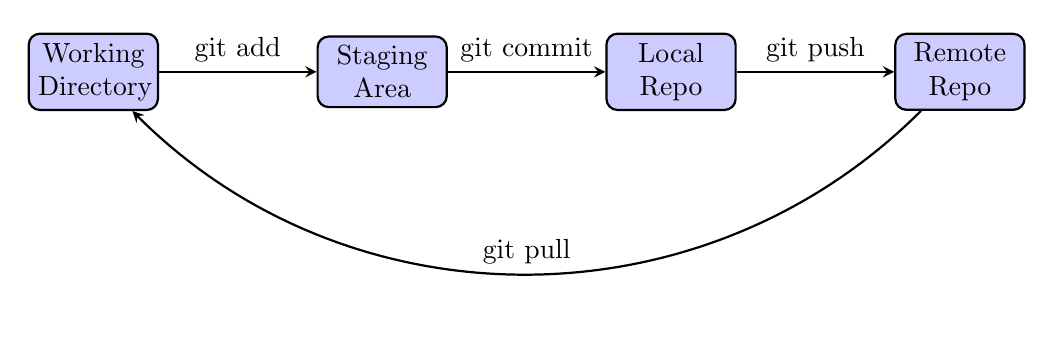
\begin{tikzpicture}[node distance=2cm, auto, thick]
    \tikzstyle{box} = [rectangle, draw, fill=blue!20, text width=4em, text centered, rounded corners, minimum height=2em]
    \tikzstyle{arrow} = [->, >=stealth]
    
    \node [box] (working) {Working\\Directory};
    \node [box, right=of working] (staging) {Staging\\Area};
    \node [box, right=of staging] (local) {Local\\Repo};
    \node [box, right=of local] (remote) {Remote\\Repo};
    
    \draw [arrow] (working) -- node {git add} (staging);
    \draw [arrow] (staging) -- node {git commit} (local);
    \draw [arrow] (local) -- node {git push} (remote);
    \draw [arrow] (remote) to [bend left=45] node[above] {git pull} (working);
\end{tikzpicture}
\end{center}

\vspace{0.3cm}
\begin{itemize}
    \item Edit files in working directory
    \item Stage changes you want to commit
    \item Commit creates permanent snapshot
    \item Push shares with collaborators
\end{itemize}
\end{frame}

\begin{frame}[fragile]{Essential Git Commands}
\begin{block}{Repository Setup}
\begin{verbatim}
git init                 # Initialize new repo
git clone <url>          # Copy remote repo
\end{verbatim}
\end{block}

\begin{block}{Daily Workflow}
\begin{verbatim}
git status               # Check current state
git add <file>           # Stage specific file
git add .                # Stage all changes
git commit -m "msg"      # Commit with message
git fetch                # Download remote changes
git pull                 # Fetch + merge changes
git push origin main     # Push to remote
git log                  # View commit history
git diff                 # See unstaged changes
\end{verbatim}
\end{block}
\end{frame}

\begin{frame}{Branching Strategy}
\textbf{Why branches?}
\begin{itemize}
    \item Isolate experimental work
    \item Develop features independently
    \item Keep main branch stable
\end{itemize}

\vspace{0.3cm}

\textbf{Common workflow:}
\begin{enumerate}
    \item Create branch for new feature: \texttt{git checkout -b feature-name}
    \item Make changes and commit
    \item Push branch: \texttt{git push -u origin feature-name}
    \item Create pull request on GitHub
    \item Review and merge
    \item Delete branch after merge
\end{enumerate}
\end{frame}

\begin{frame}{Visualizing Branches}
\begin{center}
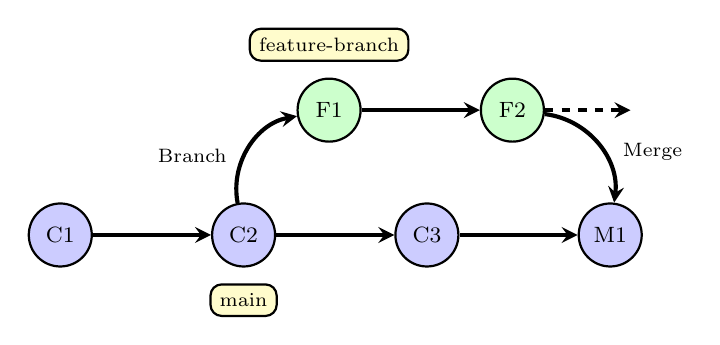
\begin{tikzpicture}[node distance=1.5cm, auto, thick]
    % Styles
    \tikzstyle{commit} = [circle, draw, fill=blue!20, minimum size=0.8cm, font=\footnotesize]
    \tikzstyle{commit_feature} = [circle, draw, fill=green!20, minimum size=0.8cm, font=\footnotesize]
    \tikzstyle{arrow} = [->, >=stealth, line width=1.5pt]
    \tikzstyle{label_box} = [rectangle, draw, fill=yellow!20, rounded corners, font=\scriptsize]

    % Main timeline
    \node [commit] (c1) {C1};
    \node [commit, right=of c1] (c2) {C2};
    \node [commit, right=of c2] (c3) {C3};
    \node [commit, right=of c3] (m1) {M1};
    
    % Feature branch
    \node [commit_feature, above right=1cm and 0.5cm of c2] (f1) {F1};
    \node [commit_feature, right=of f1] (f2) {F2};
    
    % Connections
    \draw [arrow] (c1) -- (c2);
    \draw [arrow] (c2) -- (c3);
    \draw [arrow] (c3) -- (m1);
    
    \draw [arrow] (f1) -- (f2);
    
    % Branching and Merging
    \draw [arrow] (c2) to [bend left=45] node[near start, above left, font=\scriptsize] {Branch} (f1);
    \draw [arrow] (f2) to [bend left=45] node[near end, above right, font=\scriptsize] {Merge} (m1);
    
    % Branch continues (open)
    \draw [arrow, dashed] (f2) -- ++(1.5, 0);
    
    % Labels
    \node [label_box, below=0.2cm of c2] {main};
    \node [label_box, above=0.2cm of f1] {feature-branch};
    
\end{tikzpicture}
\end{center}

\vspace{0.2cm}
\begin{itemize}
    \item \textbf{Branch}: Create a parallel timeline (\texttt{git checkout -b})
    \item \textbf{Commit}: Work on the feature branch (F1, F2)
    \item \textbf{Merge}: Combine feature history back into main (\texttt{git merge})
    \item \textit{Note: The branch remains open after merging unless deleted}
\end{itemize}
\end{frame}

\begin{frame}{Git Best Practices}
\begin{block}{Commit Messages}
\begin{itemize}
    \item Be descriptive: "Add regression analysis for Model 2"
    \item Use imperative mood: "Fix data loading bug"
    \item Reference issues: "Closes \#42"
\end{itemize}
\end{block}

\begin{block}{What to Commit}
\begin{itemize}
    \item \textcolor{green}{DO}: Source code, scripts, documentation
    \item \textcolor{green}{DO}: Raw data (if reasonable size)
    \item \textcolor{red}{DON'T}: Generated outputs (rebuild from scripts)
    \item \textcolor{red}{DON'T}: Large binary files (use Git LFS if needed)
    \item \textcolor{red}{DON'T}: Passwords or API keys
\end{itemize}
\end{block}

% \begin{block}{Commit Frequency}
% \begin{itemize}
%     \item Commit often (atomic commits)
%     \item Each commit = one logical change
%     \item Makes history easier to understand
% \end{itemize}
% \end{block}
\end{frame}

\begin{frame}[fragile]{The .gitignore File}
\textbf{What is .gitignore?}
\begin{itemize}
    \item Tells Git which files to ignore (never commit)
    \item Prevents committing generated files, credentials, or large binaries
    \item One per repository (in root directory)
\end{itemize}

\vspace{0.3cm}

\textbf{Example .gitignore for Research Projects:}
\begin{columns}
\begin{column}{0.48\textwidth}
\scriptsize
\begin{verbatim}
# Python
__pycache__/
*.pyc
.ipynb_checkpoints/
*.egg-info/

# R
.Rhistory
.RData
.Rproj.user/

\end{verbatim}
\end{column}

\begin{column}{0.48\textwidth}
\scriptsize
\begin{verbatim}
# LaTeX
*.aux
*.bbl
*.blg
*.log
*.out
*.fls
*.synctex.gz

# Generated outputs
output/
*.pdf
*.png
\end{verbatim}
\end{column}
\end{columns}

% \vspace{0.2cm}
% \textbf{Pro tip:} Use \url{gitignore.io} to generate templates for your language/tools!
\end{frame}


\begin{frame}{Common Challenges \& Solutions}

\textbf{Understanding Merge Conflicts:}
\begin{itemize}
    \item Occur when Git cannot automatically determine which version to keep
    \item Happen when the same lines of code/text are edited in different branches
    \item VS Code highlights conflicts and lets you choose which version to keep
    \item AI agents can suggest the best resolution strategy!
\end{itemize}

\vspace{0.2cm}

\textbf{Backing Up Your Work:}
\begin{itemize}
    \item You can keep your local repo in Dropbox for automatic backup
    \item Avoid sharing that Dropbox folder with co-authors unless you can really coordinate well
    % \item Use GitHub for collaboration, Dropbox only for personal backup
\end{itemize}

\vspace{0.2cm}

\begin{table}
\scriptsize
\begin{tabular}{lp{6.5cm}}
\toprule
\textbf{Challenge} & \textbf{Solution} \\
\midrule
Merge conflicts & Use VS Code conflict resolver, ask AI agent for help \\
Large files & Use .gitignore, Git LFS if needed \\
Slow Git operations & Use .gitignore for generated files \\
Lost work & Commit often, use branches \\
Unclear AI output & Refine prompts, add context \\
Reproducibility & Use Makefile, document dependencies \\
\bottomrule
\end{tabular}
\end{table}
\end{frame}

% ============================================================
% SECTION 4: GITHUB
% ============================================================
\begin{frame}[plain]
    \centering
    \vspace{1cm}
    \textbf{\Huge The Guardrails (Cloud)}
    
    \vspace{0.5cm}
    {\Large GitHub Collaboration}
    
    \vspace{1.5cm}
    
\begin{tikzpicture}
        \node[rectangle, draw=blue!60!black, fill=blue!10, very thick, minimum size=3cm, minimum width=3cm, align=center] {\Large Cloud\\Memory};
    \end{tikzpicture}
\end{frame}

\section{GitHub: Collaboration Platform}

\begin{frame}{What is GitHub?}
\begin{columns}[t]
\begin{column}[t]{0.5\textwidth}
\textbf{GitHub is...}
\begin{itemize}
    \item Web-based Git hosting
    \item Social coding platform
    \item Project management tools
    \item Collaboration infrastructure
    \item Portfolio for researchers
\end{itemize}
\end{column}

\begin{column}[t]{0.5\textwidth}
\textbf{Key Features:}
\begin{itemize}
    \item Remote repository hosting
    \item Pull requests
    \item Issues and project boards
    \item Hosts your personal Web site!
    \item Pages (documentation)
    \item Copilot (AI Agents)
\end{itemize}
\end{column}
\end{columns}

\vspace{0.5cm}
\textbf{Free for academic use!} (github.com/education)

\vspace{0.3cm}
\textbf{Demo:} Showing Github and Creating Personal Website
\end{frame}

\begin{frame}{GitHub Workflow: Issues}
\textbf{What are Issues?}
\begin{itemize}
    \item Track tasks, bugs, feature requests
    \item Organize work with labels and milestones
    \item Assign to team members
    \item Reference in commits and PRs
\end{itemize}

\vspace{0.3cm}

\textbf{Issue-Driven Development:}
\begin{enumerate}
    \item Create issue: ``Add robustness checks"
    \item Create branch: \texttt{git checkout -b issue-42-robustness}
    \item Work on feature, commit with ``Addresses \#42"
    \item Create pull request
    \item Merge and close: ``Closes \#42"
\end{enumerate}

\vspace{0.3cm}
\textbf{Demo:} Creating and assigning an issue to Github Copilot
\end{frame}

\begin{frame}{GitHub Workflow: Pull Requests}
\textbf{What are Pull Requests (PRs)?}
\begin{itemize}
    \item Propose changes to repository
    \item Enable code review before merging
    \item Discuss implementation details
    % \item Run automated tests
\end{itemize}

\vspace{0.1cm}

\textbf{PR Workflow:}

\begin{center}
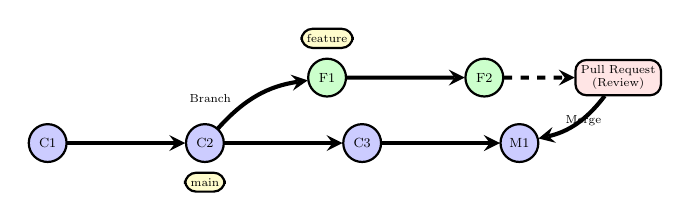
\begin{tikzpicture}[scale=0.6, transform shape, node distance=2.5cm, auto, thick]
    % Styles
    \tikzstyle{commit} = [circle, draw, fill=blue!20, minimum size=0.8cm, font=\footnotesize]
    \tikzstyle{commit_feature} = [circle, draw, fill=green!20, minimum size=0.8cm, font=\footnotesize]
    \tikzstyle{arrow} = [->, >=stealth, line width=1.5pt]
    \tikzstyle{label_box} = [rectangle, draw, fill=yellow!20, rounded corners, font=\scriptsize]
    \tikzstyle{pr_box} = [rectangle, draw, fill=red!10, rounded corners, font=\scriptsize, align=center]

    % Main timeline
    \node [commit] (c1) {C1};
    \node [commit, right=of c1] (c2) {C2};
    \node [commit, right=of c2] (c3) {C3};
    \node [commit, right=of c3] (m1) {M1};
    
    % Feature branch
    \node [commit_feature, above right=0.8cm and 2cm of c2] (f1) {F1};
    \node [commit_feature, right=of f1] (f2) {F2};
    
    % Connections
    \draw [arrow] (c1) -- (c2);
    \draw [arrow] (c2) -- (c3);
    \draw [arrow] (c3) -- (m1);
    
    \draw [arrow] (f1) -- (f2);
    
    % Branching
    \draw [arrow] (c2) to [bend left=20] node[near start, above left, font=\scriptsize] {Branch} (f1);
    
    % PR Step
    \node [pr_box, right=1.5cm of f2] (pr) {Pull Request\\(Review)};
    \draw [arrow, dashed] (f2) -- (pr);
    \draw [arrow] (pr) to [bend left=20] node[near end, above right, font=\scriptsize] {Merge} (m1);
    
    % Labels
    \node [label_box, below=0.2cm of c2] {main};
    \node [label_box, above=0.2cm of f1] {feature};
    
\end{tikzpicture}
\end{center}

\vspace{-0.3cm}
\begin{columns}[t]
    \begin{column}{0.5\textwidth}
        \footnotesize
        \begin{enumerate}
            \item Create and push feature branch
            \item Open Pull Request on GitHub
        \end{enumerate}
    \end{column}
    \begin{column}{0.5\textwidth}
        \footnotesize
        \begin{enumerate}
            \setcounter{enumi}{2}
            \item Review, discuss, and fix
            \item Merge when approved
        \end{enumerate}
    \end{column}
\end{columns}

\vspace{0.3cm}
\textbf{Demo:} Creating and reviewing a PR, did Copilot finish working?
\end{frame}

\begin{frame}{GitHub Project Boards}
\textbf{Organize Research Projects:}
\begin{itemize}
    \item Kanban-style boards
    \item Columns: To Do, In Progress, Done
    \item Link to issues and PRs
    \item Automate card movement
\end{itemize}

\vspace{0.3cm}

\textbf{Example Workflow:}
\begin{enumerate}
    \item Create project board for paper
    \item Add columns for analysis, writing, revisions
    \item Create issues for each task
    \item Move cards as work progresses
    \item Track progress visually
\end{enumerate}

\vspace{0.3cm}
\textbf{Demo:} Setting up a project board + Creating issue
\end{frame}




\begin{frame}[plain]
    \centering
    \vspace{1cm}
    \textbf{\Huge Integrations}
    
    \vspace{0.5cm}
    {\Large Putting It All Together}
    
    \vspace{1.5cm}
    
\begin{tikzpicture}
        \node[rectangle, draw=orange!60!black, fill=orange!10, very thick, minimum size=3cm, minimum width=3cm, align=center] {\Large MCP};
    \end{tikzpicture}
\end{frame}

\begin{frame}{MCP: Model Context Protocol}
\textbf{What is MCP?}
\begin{itemize}
    \item Protocol that gives AI agents access to external tools and services
    \item Enables \textit{direct interaction} with APIs (not just generating code for you)
\end{itemize}

\vspace{0.5cm}

\begin{columns}
\begin{column}{0.48\textwidth}
\textbf{Key MCP Servers:}
\scriptsize
\begin{itemize}
    \item \textbf{GitHub}: Create issues, PRs, manage boards
    \item \textbf{Playwright}: Browser automation and interaction
    \item \textbf{Filesystem} \& \textbf{Fetch}: Built-in VS Code tools
\end{itemize}

% \vspace{0.3cm}
% \normalsize
% \textbf{Without MCP:} Copy-paste \\
% \textbf{With MCP:} Automatic!
\end{column}

\begin{column}{0.48\textwidth}
\textbf{Setup (GitHub MCP):}
\scriptsize
\begin{enumerate}
    \item Install MCP server (npx)
    \item Get GitHub token
    \item Configure in Copilot settings
    \item Done!
\end{enumerate}
\end{column}
\end{columns}
\end{frame}

\begin{frame}{How AI Tools Connect: The Big Picture}
\begin{center}
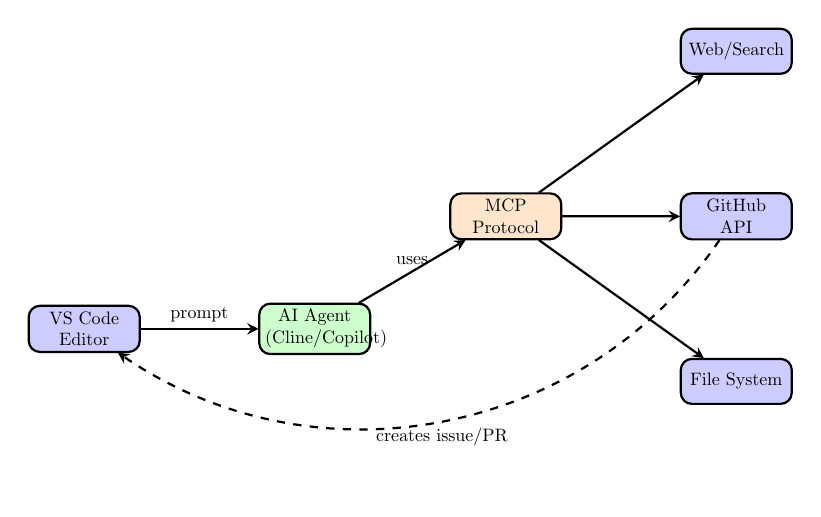
\begin{tikzpicture}[node distance=1.5cm, auto, thick, scale=0.85, every node/.style={scale=0.65}]
    \tikzstyle{box} = [rectangle, draw, fill=blue!20, text width=5.5em, text centered, rounded corners, minimum height=2.5em]
    \tikzstyle{agent} = [rectangle, draw, fill=green!20, text width=5.5em, text centered, rounded corners, minimum height=2.5em]
    \tikzstyle{tool} = [rectangle, draw, fill=orange!20, text width=5.5em, text centered, rounded corners, minimum height=2.5em]
    \tikzstyle{arrow} = [->, >=stealth, thick]
    
    \node [box] (vscode) {VS Code\\Editor};
    \node [agent, right=of vscode] (copilot) {AI Agent\\(Cline/Copilot)};
    \node [tool, above right=0.8cm and 1cm of copilot] (mcp) {MCP\\Protocol};
    \node [box, right=of mcp] (github) {GitHub\\API};
    \node [box, below=of github] (files) {File System};
    \node [box, above=of github] (web) {Web/Search};
    
    \draw [arrow] (vscode) -- node {prompt} (copilot);
    \draw [arrow] (copilot) -- node[above] {uses} (mcp);
    \draw [arrow] (mcp) -- node[above] {} (github);
    \draw [arrow] (mcp) -- node[right] {} (files);
    \draw [arrow] (mcp) -- node[right] {} (web);
    \draw [arrow, dashed] (github) to [bend left=45] node[below] {creates issue/PR} (vscode);
\end{tikzpicture}
\end{center}

\vspace{-0.8cm}
\textbf{Example Flow:}
\begin{enumerate}
    \scriptsize
    \item You: "Create issue for clustered SE analysis and add to project board"
    \item AI Agent → MCP → GitHub API → Issue created + added to board
    \item VS Code shows notification with issue link
    \item Agent can then create branch, write code, commit, create PR automatically!
\end{enumerate}
\end{frame}


\begin{frame}{Live Demo: End-to-End Example}
\textbf{Scenario:} Add a new robustness check using MCP-enabled AI agent
\vspace{0.3cm}
\begin{enumerate}
    \item Ask AI agent: ``Create issue for adding clustered SE robustness check"
    \item Agent uses GitHub MCP to create issue and add to project board
    \item Agent fetches issue details and creates branch: \texttt{feature/clustered-se}
    \item Agent uses Copilot to generate implementation code
    \item Update analysis script with AI assistance
    \item Run \texttt{make all} to regenerate outputs
    \item Agent commits changes with descriptive message
    \item Agent creates PR linking to original issue
    \item Review PR and merge to main
    \item Agent updates issue with concise description of changes and closes it
\end{enumerate}

\vspace{0.3cm}
\textbf{We'll work through this together - from idea to merged code in minutes!}
\end{frame}


% \begin{frame}{Collaboration Best Practices}
% \begin{block}{Repository Setup}
% \begin{itemize}
%     \item Clear README with setup instructions
%     % \item LICENSE file (MIT, GPL, etc.)
%     \item .gitignore for generated files
% \end{itemize}
% \end{block}

% \begin{block}{Team Workflow}
% \begin{itemize}
%     \item Never commit directly to main
%     \item All changes via pull requests
%     \item Require reviews before merging
% \end{itemize}
% \end{block}

% \begin{block}{Communication}
% \begin{itemize}
%     \item Issues for tasks and discussions
%     \item PR comments for code feedback
%     \item Wiki for documentation
% \end{itemize}
% \end{block}
% \end{frame}

\begin{frame}{Common Frictions in Academic Research}
\textbf{Integration Challenges:}

\vspace{0.2cm}

\begin{block}{Statistical Software}
\begin{itemize}
    \item \textbf{Stata/MATLAB}: Not natively integrated in VS Code
    \item \textbf{Solution}: Run through integrated terminal with commands
    \item Extensions available for syntax highlighting
    \item Execute code blocks via terminal shortcuts
\end{itemize}
\end{block}

\begin{block}{Overleaf Integration}
\begin{itemize}
    \item \textbf{Via Dropbox}: Sync local folder with Overleaf project (some lag)
    \item \textbf{Via Git}: Clone Overleaf project, push/pull changes (more control)
    \item \textbf{Via GitHub}: Sync Overleaf project with GitHub repository (requires Premium)
    \item \textbf{Alternative}: Use LaTeX Workshop extension in VS Code directly and Copy/Paste files
    % \item Trade-off: Real-time collaboration vs. local control
\end{itemize}
\end{block}

\vspace{0.1cm}
\textbf{Bottom line:} Not perfect, but workable with some adjustments!
\end{frame}

\begin{frame}{Optimum Workflow: Overleaf + VS Code}
    \centering
    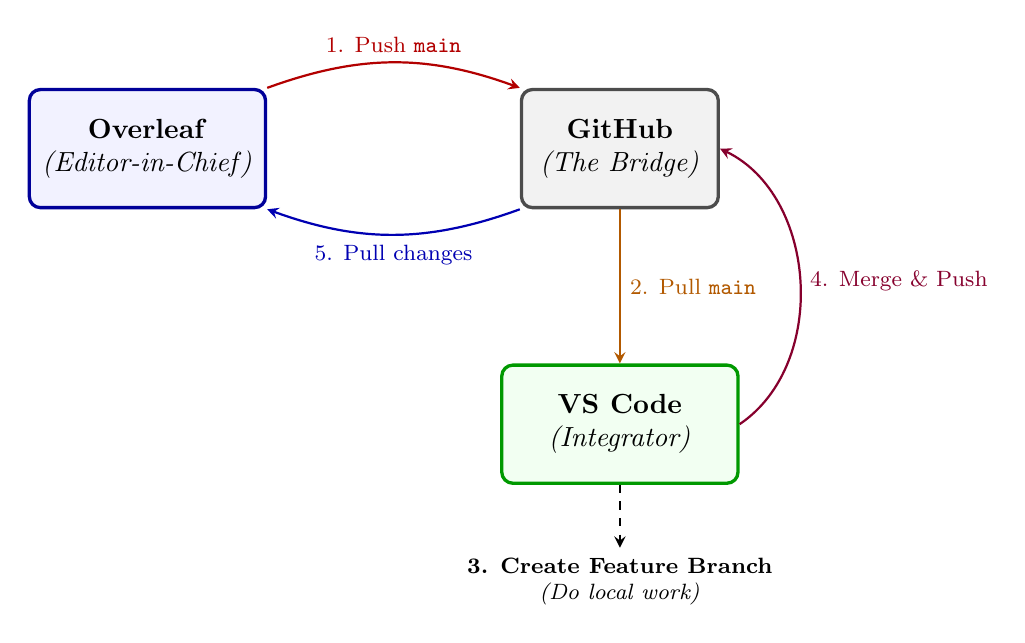
\begin{tikzpicture}[node distance=4cm, auto, >=stealth, thick]
        % Nodes
        \node[rectangle, draw=blue!60!black, fill=blue!5, very thick, minimum width=3cm, minimum height=1.5cm, rounded corners, align=center] (overleaf) {\textbf{Overleaf}\\\textit{(Editor-in-Chief)}};
        
        \node[rectangle, draw=black!70, fill=black!5, very thick, minimum width=2.5cm, minimum height=1.5cm, rounded corners, align=center, right of=overleaf, node distance=6cm] (github) {\textbf{GitHub}\\\textit{(The Bridge)}};
        
        \node[rectangle, draw=green!60!black, fill=green!5, very thick, minimum width=3cm, minimum height=1.5cm, rounded corners, align=center, below of=github, node distance=3.5cm] (local) {\textbf{VS Code}\\\textit{(Integrator)}};

        % Arrows
        % 1. Overleaf -> GitHub
        \draw[->, red!70!black] (overleaf.north east) to [bend left=20] node[above, font=\footnotesize] {1. Push \texttt{main}} (github.north west);
        
        % 5. GitHub -> Overleaf
        \draw[->, blue!70!black] (github.south west) to [bend left=20] node[below, font=\footnotesize] {5. Pull changes} (overleaf.south east);
        
        % 2. GitHub -> Local
        \draw[->, orange!70!black] (github.south) -- node[right, font=\footnotesize] {2. Pull \texttt{main}} (local.north);
        
        % 4. Local -> GitHub
        \draw[->, purple!70!black] (local.east) to [bend right=60] node[right, font=\footnotesize] {4. Merge \& Push} (github.east);

        % 3. Local work
        \node[below of=local, node distance=2cm, align=center, font=\footnotesize] (work) {\textbf{3. Create Feature Branch}\\\textit{(Do local work)}};
        \draw[dashed, ->] (local) -- (work);
    \end{tikzpicture}

    \vspace{0.3cm}
    \small
    \begin{block}{Workflow Rules}
    \begin{itemize}
        \item \textbf{Overleaf} owns \texttt{main} (authoritative draft)
        \item \textbf{Local work} happens exclusively on \texttt{feature/*} branches
        \item \textbf{Sync} often: Pull \texttt{main} before branching
    \end{itemize}
    \end{block}
\end{frame}



% ============================================================
% SECTION 6: AGENTIC AI
% ============================================================
\section{Agentic AI for Research}

% \begin{frame}{What is Agentic AI?}
% \begin{columns}[t]
% \begin{column}[t]{0.48\textwidth}
% \begin{block}{Traditional AI Assistants}
% \begin{itemize}
%     \item Respond to queries
%     \item Generate code snippets
%     \item Provide suggestions
% \end{itemize}
% \end{block}
% \end{column}

% \begin{column}[t]{0.48\textwidth}
% \begin{block}{Agentic AI}
% \begin{itemize}
%     \item Autonomous task completion
%     \item Multi-step reasoning
%     \item Context-aware assistance
% \end{itemize}
% \end{block}
% \end{column}
% \end{columns}

% \vspace{0.5cm}

% \textbf{Key Tools:}
% \begin{itemize}
%     \item GitHub Copilot (local \& cloud)
%     \item VS Code Chat modes
%     \item Cline + Continue (offline capable!)
%     \item Cursor, Windsurf
% \end{itemize}
% \end{frame}

% \begin{frame}{GitHub Copilot Overview}
% \begin{columns}
% \begin{column}{0.5\textwidth}
% \textbf{Copilot Features:}
% \begin{itemize}
%     \item Code completion
%     \item Chat interface
%     \item Inline suggestions
%     \item Whole function generation
%     \item Documentation writing
%     \item Code explanation
% \end{itemize}
% \end{column}

% \begin{column}{0.5\textwidth}
% \textbf{Use Cases:}
% \begin{itemize}
%     \item Write boilerplate code
%     \item Debug errors
%     \item Refactor functions
%     \item Generate tests
%     \item Write docstrings
%     \item Translate code
% \end{itemize}
% \end{column}
% \end{columns}

% \vspace{0.5cm}

% \textbf{Free for students and educators!} \\
% Apply at: \url{education.github.com}
% \end{frame}



% \begin{frame}{AI-Assisted Workflows: Cloud}
% \textbf{GitHub Copilot Workspace / Claude Code / Codex / Jules (Cloud):}
% \begin{itemize}
%     \item Work on issues directly in browser
%     \item AI proposes implementation plan
%     \item Review and refine suggestions
%     \item Create PR automatically
%     \item Collaborate asynchronously!
% \end{itemize}

% \vspace{0.3cm}

% \textbf{Use Cases:}
% \begin{itemize}
%     \item Quick fixes from mobile/tablet
%     \item Delegate tasks to AI agent
%     \item Review AI-generated solutions
% \end{itemize}

% \vspace{0.3cm}
% \textbf{Demo:} Creating issue and using Copilot Workspace and Codex
% \end{frame}

\begin{frame}{Complementary Research Tools}
\begin{table}
\small
\begin{tabular}{lp{6cm}}
\toprule
\textbf{Tool} & \textbf{Purpose} \\
\midrule
\textbf{Refine} & AI-powered writing revision and style improvement \\
(refine.ink) & Interactive editing with suggestions \\
\midrule
\textbf{NotebookLM} & Structured reading and note-taking \\
(Google) & Create study guides from papers \\
         & Create academic podcasts! \\
\midrule
\textbf{Elicit} & Literature discovery and synthesis \\
& Extract data from papers \\
\midrule
\textbf{GPT/Claude/Gemini} & General research assistance \\
& Draft writing, brainstorming \\
\bottomrule
\end{tabular}
\end{table}

\vspace{0.2cm}
\textbf{Integration:} Use alongside Git/GitHub workflow for complete research pipeline
\end{frame}

% \begin{frame}{AI Best Practices}
% \begin{block}{DO:}
% \begin{itemize}
%     \item Review all AI-generated code
%     \item Test suggestions before committing
%     \item Understand what the code does
%     \item Use AI to learn new techniques
%     \item Iterate on prompts for better results
% \end{itemize}
% \end{block}

% \begin{block}{DON'T:}
% \begin{itemize}
%     \item Blindly accept all suggestions
%     \item Share sensitive data with AI
%     \item Rely on AI for critical decisions
%     % \item Forget to cite AI assistance (if required)
%     \item Use AI to write entire papers
% \end{itemize}
% \end{block}

% \vspace{0.2cm}
% \textbf{Remember:} AI is a tool, not a replacement for thinking!
% \end{frame}



% \begin{frame}{Using AI APIs in Your Code}
% \textbf{When to Use AI APIs Directly:}
% \begin{itemize}
%     \item Automate repetitive data processing tasks (classify text, extract entities)
%     \item Generate synthetic data for testing or augmentation
%     \item Create automated reports or summaries from analysis results
%     % \item Build custom research tools with AI capabilities
% \end{itemize}

% \vspace{0.3cm}

% \begin{columns}
% \begin{column}{0.48\textwidth}
% \textbf{Example: OpenAI API}
% \begin{itemize}
%     \item Text generation/completion
%     \item Code generation
%     \item Data classification
%     \item Embeddings for similarity
% \end{itemize}
% \end{column}

% \begin{column}{0.48\textwidth}
% \textbf{Example: Anthropic Claude}
% \begin{itemize}
%     \item Long document analysis
%     \item Complex reasoning tasks
%     \item JSON mode for structured output
%     \item Vision for image analysis
% \end{itemize}
% \end{column}
% \end{columns}

% \vspace{0.3cm}

% \textbf{Best Practice:} Store API keys in environment variables, never commit them to Git!
% \end{frame}


% ============================================================
% SECTION 7: PUTTING IT ALL TOGETHER
% ============================================================
% \section{Putting It All Together}

% \begin{frame}{Complete Research Workflow}
% \begin{columns}
% \begin{column}{0.48\textwidth}
% \textbf{1. Setup}
% \begin{itemize}
%     \item Clone template repository
%     \item Set up Python environment
%     \item Configure VS Code
% \end{itemize}

% \textbf{2. Development}
% \begin{itemize}
%     \item Create issues for tasks
%     \item Work in feature branches
%     \item Use AI for code generation
%     \item Commit regularly
% \end{itemize}
% \end{column}

% \begin{column}{0.48\textwidth}
% \textbf{3. Collaboration}
% \begin{itemize}
%     \item Push branches to GitHub
%     \item Create pull requests
%     \item Review code
%     \item Merge to main
% \end{itemize}

% \textbf{4. Publication}
% \begin{itemize}
%     \item Run \texttt{make all}
%     \item Compile paper and slides 
%     \item Share repository with paper
% \end{itemize}
% \end{column}
% \end{columns}
% \end{frame}



\begin{frame}{Next Steps}
\textbf{First:}
\begin{enumerate}
    \item Fork/clone workshop template repository
    \item Install VS Code and extensions
    \item Set up GitHub account (education benefits)
    \item Practice basic Git commands
    \item Run \texttt{make all} to build template
    \item Ask your favorite AI agent to explain any concepts from the slides you don't understand
\end{enumerate}

\vspace{0.3cm}

\textbf{Second:}
\begin{itemize}
    \item Apply workflow to a small project
    \item Create repository for current research
    \item Experiment with Copilot
    \item Set up project board
\end{itemize}

\end{frame}

\begin{frame}{Resources}
\begin{block}{Documentation}
\begin{itemize}
    \item Git: \url{git-scm.com/doc}
    \item GitHub: \url{docs.github.com}
    \item VS Code: \url{code.visualstudio.com/docs}
\end{itemize}
\end{block}

\begin{block}{Learning}
\begin{itemize}
    \item GitHub Skills: \url{skills.github.com}
    \item Software Carpentry: \url{software-carpentry.org}
\end{itemize}
\end{block}

\begin{block}{Workshop Materials}
\begin{itemize}
    \item Template: \url{github.com/tlarroucau/AI_workshop}
    \item Slides: \texttt{tex/slides/}
\end{itemize}
\end{block}
\end{frame}

\begin{frame}{Behind the Scenes: Meta Moment}
\begin{center}
\Large
    \textbf{This ENTIRE workshop was created with ONE prompt and SOME hours of edits!}
\end{center}

% \vspace{0.2cm}

% \begin{columns}
% \begin{column}{0.48\textwidth}
% \scriptsize
% \textbf{Tools Used:}
% \begin{itemize}
%     \item VS Code + GitHub Copilot
%     \item Git \& GitHub (version control)
%     \item LaTeX Workshop (slides)
%     \item Python + Matplotlib (sample data)
%     \item Makefile (automation)
%     \item AI agents (Copilot Chat)
% \end{itemize}
% \end{column}

% \begin{column}{0.48\textwidth}
% \scriptsize
% \textbf{Initial Prompt to AI:}
% \begin{quote}
% \textit{"Create a reproducible research project template for an ASU workshop on Git, GitHub, and VS Code with Agentic AI. Include: Python analysis scripts, LaTeX paper/slides, sample data pipeline, Makefile automation, and comprehensive documentation."}
% \end{quote}
% \end{column}
% \end{columns}

% \vspace{0.3cm}

% \textbf{The Result:}
% \begin{itemize}
%     \item Full repository structure generated in minutes
%     \item AI helped refine slides, code, and documentation
%     \item Version controlled from day one
%     \item Reproducible workflow demonstrated live
% \end{itemize}

% \vspace{0.2cm}
% \centering
% \small
% \textbf{This is the future of research productivity!}
\end{frame}



\begin{frame}{Questions?}
\begin{center}
\Large
Thank you for attending!

\vspace{1cm}

\normalsize
\textbf{Contact:} Tomas.Larroucau@asu.edu

\vspace{0.5cm}

\textbf{Template Repository:} \\
\url{github.com/tlarroucau/AI_workshop}

% \vspace{0.5cm}

% \textbf{Office Hours:} By appointment
\end{center}
\end{frame}





% ============================================================
% APPENDIX
% ============================================================
\appendix
\section{Appendix}

\begin{frame}[fragile]{The Makefile Approach}
\hypertarget{appendix-makefile}{}
\begin{columns}[t]
\begin{column}{0.48\textwidth}
\textbf{What is a Makefile?}

A recipe file that automates your workflow. You define \textit{targets}, their \textit{dependencies}, and the \textit{commands} to run.

\vspace{0.2cm}

\begin{block}{Syntax}
\begin{verbatim}
target: dependencies
    command to run
\end{verbatim}
\end{block}

Then type \texttt{make target} in the terminal.

\vspace{0.3cm}

\textbf{Why it matters for AI:} When agents modify your code, \texttt{make all} re-runs the full pipeline --- ensuring reproducibility even after AI-generated changes.
\end{column}

\begin{column}{0.48\textwidth}
\begin{block}{Example}
\scriptsize
\begin{verbatim}
DATA = data/raw/sample_data.csv
OPTS = --robust --output output/

all: analysis paper

analysis: $(DATA)
    python scripts/analysis.py $(OPTS)

paper:
    cd tex/paper && latexmk paper

clean:
    rm -rf output/*
\end{verbatim}
\end{block}

\vspace{0.2cm}
\normalsize
\textbf{Demo:} \texttt{make all}
\end{column}
\end{columns}

\vspace{0.3cm}
\hyperlink{main-project-structure}{\beamerbutton{Back to Project Structure}}
\end{frame}


\end{document}
